% magick -quality 90 -density 1200 $input -resize 25% -trim $output

\documentclass{standalone}
\usepackage{tikz}

\usetikzlibrary{calc,math}


\begin{document}

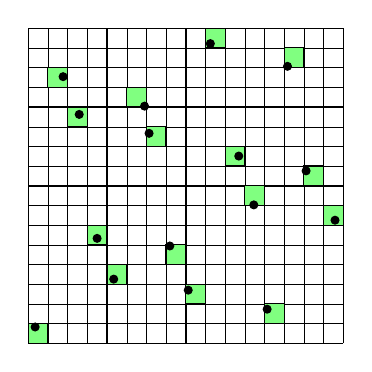
\begin{tikzpicture}
  \draw[ultra thin,xstep=0.25cm,ystep=0.25cm] (0,0) grid (4,4);
  \draw[thin] (0,0) grid (4,4);

  \foreach \i in {1,2,3,4} {
    \foreach \j in {1,2,3,4} {
      \tikzmath{
        int \k;
        \k = (\i - 1) * 4 + (\j - 1);
        \k = mod(\k * 7, 16);
        int \ii;
        \ii = int(floor(\k / 4));
        int \jj;
        \jj = mod(\k, 4);
        real \x;
        real \y;
        real \dx;
        real \dy;
        \x = \i - 1 + \jj * 0.25;
        \y = \j - 1 + \ii * 0.25;
        \dx = random() * 0.25;
        \dy = random() * 0.25;
      }

      \draw[fill=green!50] (\x, \y) rectangle ++(.25, .25);
      \draw[fill=black] ($ (\x, \y) + (\dx, \dy) $) circle [radius=0.05cm];
    }
  }
\end{tikzpicture}

\end{document}